% IEEE Conference-style Thesis Proposal
% Compile: pdflatex thesis_proposal.tex && pdflatex thesis_proposal.tex
\documentclass[conference]{IEEEtran}

% ---- Packages ----
\usepackage{cite}
\usepackage{amsmath,amssymb,amsfonts}
\usepackage{algorithmic}
\usepackage{graphicx}
\usepackage{textcomp}
\usepackage{xcolor}
\usepackage{booktabs}
\usepackage{multirow}
\usepackage{hyperref}
\usepackage{url}
\usepackage{tikz}
\usepackage{pgfplots}
\pgfplotsset{compat=1.18}
\usetikzlibrary{shapes.geometric, arrows.meta, positioning, fit, backgrounds, calc, patterns, decorations.pathreplacing}
\graphicspath{{images/}}

\renewcommand{\arraystretch}{1.15}

% TikZ styles
\tikzset{
    block/.style={rectangle, draw, fill=blue!8, text width=2.2cm, text centered, rounded corners, minimum height=0.8cm, font=\footnotesize},
    blockwide/.style={rectangle, draw, fill=blue!8, text width=3.0cm, text centered, rounded corners, minimum height=0.8cm, font=\footnotesize},
    sensor/.style={rectangle, draw, fill=green!15, text width=1.8cm, text centered, rounded corners, minimum height=0.7cm, font=\footnotesize},
    model/.style={rectangle, draw, fill=orange!20, text width=2.4cm, text centered, rounded corners, minimum height=0.8cm, font=\footnotesize},
    output/.style={rectangle, draw, fill=red!12, text width=2.2cm, text centered, rounded corners, minimum height=0.8cm, font=\footnotesize},
    arrow/.style={-Stealth, thick},
    dashedarrow/.style={-Stealth, thick, dashed},
    layerbox/.style={draw, dashed, rounded corners, inner sep=6pt},
}

\begin{document}

\title{Green-AI: Autonomous Post-Harvest Ripening Control via Distilled Reinforcement Learning on the Edge}

\author{
\IEEEauthorblockN{Tristan O. Jadman}
\IEEEauthorblockA{
Department of Computer Engineering\\and Mechatronics \\
\textit{Undergraduate Thesis}}
\and
\IEEEauthorblockN{Engr. Francis Jann Alagon}
\IEEEauthorblockA{
Department of Computer Engineering\\and Mechatronics \\
\textit{Thesis Adviser}}
}

\maketitle

% ==============================================================
\begin{abstract}
Post-harvest losses account for 20--40\% of tomato production in developing countries, driven by the absence of affordable, intelligent decision-support systems. Existing IoT solutions provide passive monitoring without autonomous action, while cloud-based reinforcement learning (RL) systems require expensive infrastructure and continuous connectivity. This thesis proposes \textit{Edge-RL}, a novel system that deploys a complete RL-based decision pipeline---from visual perception to autonomous harvest timing---entirely on a \$33 ESP32-S3 microcontroller. The system integrates a MobileNetV2-based ripeness classifier (INT8, $\sim$300\,KB) with a distilled Deep Q-Network policy (INT8, $\sim$35\,KB) trained via sim-to-real transfer on a physics-based digital twin. By leveraging ESP-DL's hardware-optimized inference ($\sim$10$\times$ faster than TFLite Micro), Edge-RL achieves sub-2-second combined inference for ripeness classification and harvest timing decisions. This work presents the first demonstration of a complete sim-to-edge RL pipeline for agricultural post-harvest optimization, offering smallholder farmers an autonomous, connectivity-independent alternative to commercial ripening infrastructure costing \$10,000--\$50,000.
\end{abstract}

\begin{IEEEkeywords}
Edge intelligence, reinforcement learning, post-harvest management, ESP32-S3, sim-to-real transfer, model compression, precision agriculture, digital twin
\end{IEEEkeywords}

% ==============================================================
\section{Introduction}
\label{sec:introduction}

Global food systems lose approximately 14\% of production between harvest and retail~\cite{fao2019}, with post-harvest losses in developing countries escalating to 20--40\% for perishable crops such as tomatoes~\cite{kader2005}. These losses are not merely agricultural; they represent a \$400 billion annual economic burden and a significant barrier to food security for the estimated 500 million smallholder farming households that produce over 80\% of food consumed in developing economies~\cite{worldbank2020}.

The tomato supply chain is particularly vulnerable. Ripening is a temperature-dependent, irreversible biochemical process that demands precise timing decisions: harvest too early and fruit quality suffers; harvest too late and shelf life is insufficient for market delivery. Commercial ripening facilities address this with controlled atmosphere storage, real-time monitoring, and expert-driven decision protocols---at costs of \$10,000--\$50,000 per facility~\cite{prasad2018}. For smallholder farmers earning <\$2,000 annually, this infrastructure is entirely inaccessible.

Three categories of technological solutions have emerged, each with fundamental limitations:

\textbf{1) Passive IoT monitoring.} Sensor-based systems report environmental conditions (temperature, humidity) but provide no decision support~\cite{ray2017}. They answer ``what is the temperature?'' but not ``when should I harvest given my target delivery date?''

\textbf{2) Cloud-based agricultural RL.} Reinforcement learning has demonstrated strong results in greenhouse climate control~\cite{chen2022greenhouse} and irrigation scheduling~\cite{yang2020irrigation}. However, these systems require continuous cloud connectivity, incur ongoing operational costs, and introduce latency incompatible with edge deployment in rural settings with intermittent connectivity.

\textbf{3) Edge classification systems.} Recent work deploys lightweight CNNs on microcontrollers for crop disease detection~\cite{li2021edgeai} and quality grading. These systems classify but do not \textit{decide}---they lack the sequential decision-making capability needed for dynamic optimization over time.

\textit{Edge-RL bridges all three gaps simultaneously}: it provides autonomous decision-making (not just monitoring), runs entirely at the edge (no cloud dependency), and integrates both perception and sequential optimization (not just classification)---on a \$33 microcontroller.

\subsection{Research Questions}
\label{sec:research_questions}

To address the limitations of existing IoT and Cloud-RL solutions, this study investigates the following questions:

\begin{enumerate}
    \item[\textbf{RQ1.}] To what extent can Deep Q-Network policies be compressed via knowledge distillation for real-time inference on resource-constrained microcontrollers without significant loss in decision optimality? (Aligned with \textbf{O1})

    \item[\textbf{RQ2.}] How effective is domain randomization within a physics-based digital twin in facilitating zero-shot transfer of harvest timing policies to physical environments with stochastic sensor noise? (Aligned with \textbf{O2})

    \item[\textbf{RQ3.}] Does an autonomous Edge-RL system outperform fixed-schedule heuristic control in balancing post-harvest quality preservation against energy consumption and operational viability? (Aligned with \textbf{O3})
\end{enumerate}

\subsection{Research Objectives}

This study aims to demonstrate:

\begin{enumerate}
    \item[\textbf{O1.}] \textit{Edge RL feasibility}: A distilled RL policy and a quantized vision model can jointly execute on ESP32-S3 hardware with sub-2-second total inference latency and $\geq$85\% ripeness classification accuracy.

    \item[\textbf{O2.}] \textit{Sim-to-real policy transfer}: An RL harvest timing policy trained entirely in a physics-based digital twin with domain randomization transfers to real sensor data, outperforming fixed-rule baselines.

    \item[\textbf{O3.}] \textit{Operational Efficiency and Viability}: Evaluate the trade-off between harvest quality preservation and energy consumption of the proposed edge intelligence system compared to traditional fixed-schedule methods, demonstrating economic viability for smallholder applications.
\end{enumerate}

\subsection{Contributions}

\begin{enumerate}
    \item The \textbf{first sim-to-edge RL pipeline for post-harvest agriculture} on a sub-\$50 microcontroller, demonstrating that autonomous sequential decision-making is viable at the extreme edge of computing.

    \item A \textbf{physics-based tomato ripening digital twin} implementing a temperature-dependent ODE model with domain randomization, enabling RL policy training without physical crop cycles.

    \item A \textbf{complete open-source reference implementation} of the edge RL pipeline---from training scripts to quantized firmware---enabling reproducibility and extension to other crops.
\end{enumerate}

\subsection{Conceptual Framework}
\label{sec:framework}

The study follows an Input-Process-Output (IPO) model, as illustrated in Fig.~\ref{fig:framework}.

\begin{figure}[htbp]
\centering
\resizebox{\columnwidth}{!}{%
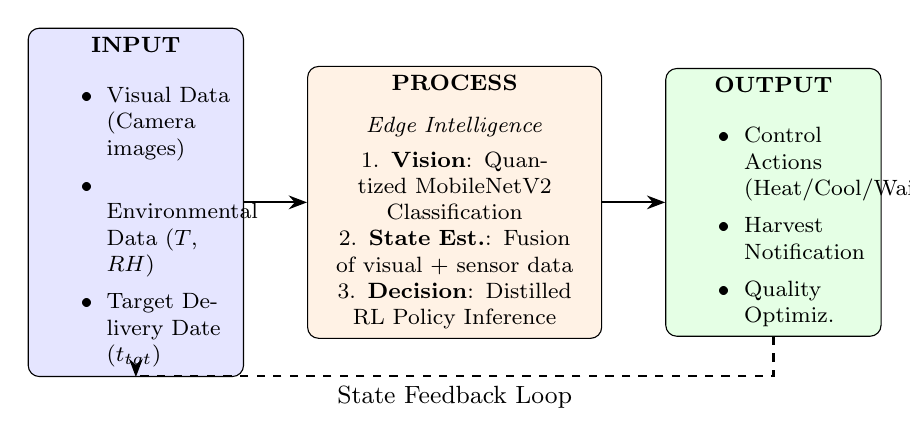
\begin{tikzpicture}[node distance=0.5cm, font=\small]
    % INPUT
    \node[block, fill=blue!10, text width=2.5cm, minimum height=3cm] (input) {
        \textbf{INPUT}\\[0.3cm]
        \begin{itemize}
            \item Visual Data (Camera images)
            \item Environmental Data ($T$, $RH$)
            \item Target Delivery Date ($t_{tgt}$)
        \end{itemize}
    };

    % PROCESS
    \node[block, fill=orange!10, text width=3.5cm, minimum height=3cm, right=0.8cm of input] (process) {
        \textbf{PROCESS}\\[0.2cm]
        \textit{Edge Intelligence}\\[0.1cm]
        1. \textbf{Vision}: Quantized MobileNetV2 Classification\\
        2. \textbf{State Est.}: Fusion of visual + sensor data\\
        3. \textbf{Decision}: Distilled RL Policy Inference
    };

    % OUTPUT
    \node[block, fill=green!10, text width=2.5cm, minimum height=3cm, right=0.8cm of process] (output) {
        \textbf{OUTPUT}\\[0.3cm]
        \begin{itemize}
            \item Control Actions (Heat/Cool/Wait)
            \item Harvest Notification
            \item Quality Optimiz.
        \end{itemize}
    };

    % Arrows
    \draw[arrow] (input) -- (process);
    \draw[arrow] (process) -- (output);
    
    % Feedback
    \draw[arrow, dashed] (output.south) -- ++(0,-0.5) -| (input.south) node[near start, below] {State Feedback Loop};

\end{tikzpicture}
}
\caption{Conceptual Framework of the Edge-RL System. The system processes multi-modal inputs through sequential on-device AI models to produce optimal control actions, forming a closed-loop feedback system.}
\label{fig:framework}
\end{figure}

The \textbf{Input} consists of raw visual data captured by the OV2640 camera and environmental readings from the DHT22 sensor. The \textbf{Process} stage involves the core edge intelligence: first, the quantized vision model classifies the tomato's ripeness stage; second, this visual state is fused with sensor data; third, the distilled RL policy determines the optimal action. The \textbf{Output} is the actuation command (heater/cooler relay) or a harvest notification, which in turn affects the physical environment, creating a feedback loop.

% ==============================================================
\section{Related Work}
\label{sec:related_work}

\subsection{Edge AI in Precision Agriculture}

The deployment of neural networks on microcontrollers---termed \textit{TinyML}~\cite{warden2019tinyml}---has matured rapidly. Banbury et al.~\cite{banbury2021mlperf} established standardized benchmarks for MCU inference, revealing that optimized runtimes can achieve real-time classification on devices with $<$512\,KB SRAM. Lin et al.~\cite{lin2020mcunet} demonstrated that co-designing neural architectures with memory-aware search (MCUNet) achieves ImageNet-level accuracy on ARM Cortex-M class devices, pushing the boundary of what edge AI can accomplish.

For agricultural deployments specifically, ESP-DL~\cite{espdl2024}---Espressif's native deep learning library for the ESP32-S3---achieves approximately 10$\times$ inference speedup over TensorFlow Lite Micro by exploiting the S3's vector instructions, dual-core scheduling, and automated SRAM/PSRAM memory planning. Prior work has demonstrated plant disease classification~\cite{li2021edgeai}, fruit quality grading~\cite{zhang2021tomato}, and soil monitoring on ESP32 platforms.

Tomato classification in particular has been extensively studied. Phan et al.~\cite{phan2023tomato} achieved 98--100\% accuracy using CNN architectures (ResNet-50/101) with YOLOv5 for simultaneous detection and classification of ripeness stages. However, these results use server-class GPUs for inference. On-device tomato classification at the microcontroller level remains underexplored, and existing edge systems are exclusively limited to \textit{single-shot classification}---they produce a label at one point in time but do not perform \textit{sequential decision-making} that considers the temporal dynamics of biological processes.

\subsection{Reinforcement Learning for Agricultural Optimization}

RL has been applied to greenhouse climate control, where agents learn temperature and humidity setpoint policies that outperform fixed-rule controllers~\cite{chen2022greenhouse}. Hemming et al.~\cite{hemming2020greenhouse} at Wageningen University demonstrated that deep RL (DDPG) can reduce energy consumption by 15--20\% while maintaining crop yield in Dutch greenhouse tomato production. Deep RL approaches---PPO, SAC---have been explored for irrigation scheduling~\cite{yang2020irrigation}, nutrient management, and crop planning.

Overweg et al.~\cite{overweg2021cropgym} introduced CropGym, a standardized RL environment for crop management that enables reproducible comparison of RL algorithms on agricultural tasks. Tao et al.~\cite{tao2019digital} surveyed the broader digital twin paradigm in industry, establishing the theoretical framework for coupling physical agricultural processes with virtual simulation environments for RL training.

These works establish RL's capability for agricultural optimization, but all operate with cloud or server-based inference. The computational and connectivity requirements of existing agricultural RL systems limit deployment to well-resourced commercial operations. Our work extends this paradigm by demonstrating that RL policy inference can be performed \textit{directly on the microcontroller} through policy distillation and INT8 quantization. DQN~\cite{mnih2015dqn} is preferred over continuous-action algorithms because the four agricultural actions (maintain, heat, cool, harvest) are inherently discrete interventions, not points on a continuous scale.

\subsection{Sim-to-Real Transfer}

Sim-to-real transfer---training policies entirely in simulation and deploying them in the physical world---is well-established in robotics~\cite{tobin2017sim2real}. Domain randomization, which systematically varies simulator parameters during training, is a key technique for bridging the reality gap~\cite{peng2018simtoreal}. Andrychowicz et al.~\cite{andrychowicz2020matters} demonstrated with OpenAI's Rubik's cube manipulation that automatic domain randomization (ADR) enables zero-shot transfer of complex policies, establishing that sufficiently diverse simulation can substitute for real-world data entirely. Zhao et al.~\cite{zhao2020simtoreal} provide a comprehensive survey of sim-to-real methods, categorizing approaches into domain randomization, domain adaptation, and system identification.

While extensively studied for robotic manipulation and locomotion, sim-to-real methods have received limited attention in agricultural contexts. Agricultural processes differ fundamentally from robotic tasks: they operate on biological timescales (days rather than seconds), involve irreversible state transitions (ripening cannot be undone), and feature significant natural variability. This thesis applies sim-to-real techniques to post-harvest management, constructing a calibrated digital twin based on established ripening kinetics~\cite{saltveit2005} with domain randomization across cultivar-specific parameters.

\subsection{Model Compression for Microcontrollers}

Han et al.~\cite{han2016deep} established the foundational three-stage compression pipeline---pruning, quantization, and Huffman coding---achieving 35--49$\times$ compression on AlexNet and VGGNet without accuracy loss. INT8 post-training quantization alone reduces model size by 4$\times$ from FP32 with minimal accuracy degradation~\cite{jacob2018quantization}. Gholami et al.~\cite{gholami2021survey} provide a comprehensive survey of quantization methods, comparing post-training quantization (PTQ) and quantization-aware training (QAT) across architectures.

Knowledge distillation~\cite{hinton2015distilling} trains compact student networks to approximate larger teacher networks, enabling further compression. Ruffy and Chahal~\cite{ruffy2019distilling} applied knowledge distillation specifically to RL policies, demonstrating that distilled policies can retain $>$95\% of teacher performance at a fraction of the parameter count---a result central to our edge RL approach. Together, these techniques make it possible to deploy models designed for GPU inference on microcontrollers with $<$512\,KB of SRAM.

\subsection{Research Gap}

Table~\ref{tab:gap} summarizes the capabilities of existing approaches against Edge-RL, identifying the gap this thesis addresses.

\begin{table}[htbp]
\caption{Capability Comparison: Edge-RL vs. Existing Approaches}
\label{tab:gap}
\centering
\begin{tabular}{@{}p{1.7cm}cccc@{}}
\toprule
\textbf{Capability} & \textbf{IoT} & \textbf{Edge AI} & \textbf{Cloud RL} & \textbf{Edge-RL} \\
\midrule
Sensing & \checkmark & \checkmark & \checkmark & \checkmark \\
Classification & & \checkmark & \checkmark & \checkmark \\
Sequential decisions & & & \checkmark & \checkmark \\
Offline operation & \checkmark & \checkmark & & \checkmark \\
Sub-\$50 BOM & \checkmark & \checkmark & & \checkmark \\
No cloud needed & \checkmark & \checkmark & & \checkmark \\
\bottomrule
\end{tabular}
\vspace{2pt}
{\scriptsize Edge-RL is the only approach that provides all six capabilities simultaneously.}
\end{table}

% ==============================================================
\section{System Architecture}
\label{sec:architecture}

Edge-RL employs a two-layer architecture: a development host for model training and an ESP32-S3 edge device for real-time inference. The training layer operates offline, producing quantized model artifacts; the edge layer operates autonomously without network connectivity. Fig.~\ref{fig:architecture} illustrates the complete system.

% ---- Figure: System Architecture (two-column) ----
\begin{figure*}[htbp]
\centering
\resizebox{\textwidth}{!}{%
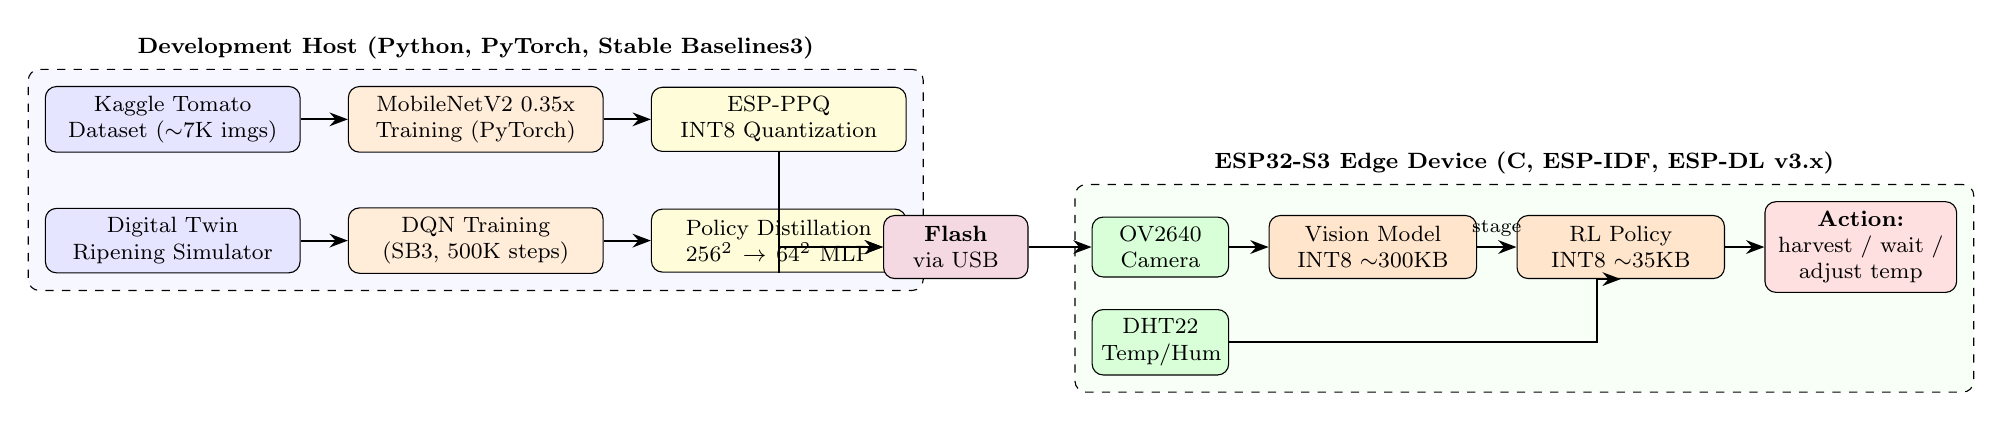
\begin{tikzpicture}[node distance=0.6cm and 0.5cm, font=\footnotesize]

    % === DEVELOPMENT HOST ===
    \node[blockwide, fill=blue!10] (kaggle) {Kaggle Tomato\\Dataset ($\sim$7K imgs)};
    \node[blockwide, fill=orange!15, right=0.6cm of kaggle] (visiontrain) {MobileNetV2 0.35x\\Training (PyTorch)};
    \node[blockwide, fill=yellow!15, right=0.6cm of visiontrain] (quantv) {ESP-PPQ\\INT8 Quantization};

    \node[blockwide, fill=blue!10, below=0.7cm of kaggle] (digtwin) {Digital Twin\\Ripening Simulator};
    \node[blockwide, fill=orange!15, right=0.6cm of digtwin] (dqntrain) {DQN Training\\(SB3, 500K steps)};
    \node[blockwide, fill=yellow!15, right=0.6cm of dqntrain] (distill) {Policy Distillation\\$256^2 \rightarrow 64^2$ MLP};

    \draw[arrow] (kaggle) -- (visiontrain);
    \draw[arrow] (visiontrain) -- (quantv);
    \draw[arrow] (digtwin) -- (dqntrain);
    \draw[arrow] (dqntrain) -- (distill);

    % === FLASH ===
    \node[block, fill=purple!15, text width=1.6cm, below right=0.8cm and -0.3cm of quantv] (flash) {\textbf{Flash}\\via USB};
    \draw[arrow] (quantv.south) |- (flash.west);
    \draw[arrow] (distill.south) |- (flash.west);

    % === ESP32-S3 ===
    \node[sensor, right=0.8cm of flash, fill=green!15, text width=1.5cm] (camera) {OV2640\\Camera};
    \node[model, right=0.5cm of camera] (vmodel) {Vision Model\\INT8 $\sim$300KB};
    \node[model, right=0.5cm of vmodel] (rlpol) {RL Policy\\INT8 $\sim$35KB};
    \node[output, right=0.5cm of rlpol] (action) {\textbf{Action:}\\harvest / wait /\\adjust temp};

    \node[sensor, fill=green!15, text width=1.5cm, below=0.4cm of camera] (dht) {DHT22\\Temp/Hum};

    \draw[arrow] (flash) -- (camera);
    \draw[arrow] (camera) -- (vmodel);
    \draw[arrow] (vmodel) -- (rlpol) node[midway, above, font=\scriptsize] {stage};
    \draw[arrow] (rlpol) -- (action);
    \draw[arrow] (dht.east) -| ([xshift=-0.3cm]rlpol.south) -- (rlpol.south);

    % Bounding boxes
    \begin{scope}[on background layer]
        \node[layerbox, fill=blue!3, fit=(kaggle)(visiontrain)(quantv)(digtwin)(dqntrain)(distill), label={[font=\footnotesize\bfseries]above:Development Host (Python, PyTorch, Stable Baselines3)}] {};
        \node[layerbox, fill=green!3, fit=(camera)(vmodel)(rlpol)(action)(dht), label={[font=\footnotesize\bfseries]above:ESP32-S3 Edge Device (C, ESP-IDF, ESP-DL v3.x)}] {};
    \end{scope}

\end{tikzpicture}
}%
\caption{Edge-RL system architecture. Two parallel pipelines produce quantized models flashed to the ESP32-S3. The edge device combines camera-based ripeness classification with sensor-informed RL decisions for autonomous harvest timing.}
\label{fig:architecture}
\end{figure*}

\subsection{Hardware Platform}

The edge device is built around the ESP32-S3-DevKitC-1 (N16R8) with 16\,MB flash, 8\,MB PSRAM, and 512\,KB internal SRAM. Table~\ref{tab:hardware} lists the complete bill of materials at \$33.

\begin{table}[htbp]
\caption{Hardware Bill of Materials}
\label{tab:hardware}
\centering
\begin{tabular}{@{}llr@{}}
\toprule
\textbf{Component} & \textbf{Model} & \textbf{Cost} \\
\midrule
MCU & ESP32-S3-DevKitC-1 (N16R8) & \$8 \\
Camera & OV2640 (2MP, 320$\times$240) & \$5 \\
Sensor & DHT22 ($\pm$0.5°C, $\pm$2\% RH) & \$3 \\
LED Indicator & WS2812B strip (8 LEDs) & \$2 \\
Power & USB-C cable + adapter & \$5 \\
Miscellaneous & Breadboard, wires, enclosure & \$10 \\
\midrule
\textbf{Total} & & \textbf{\$33} \\
\bottomrule
\end{tabular}
\end{table}

\subsection{Memory Architecture}

Fig.~\ref{fig:memory} shows the memory allocation strategy, which is critical for fitting both models within the ESP32-S3's heterogeneous memory hierarchy. The RL policy ($\sim$35\,KB) resides in fast internal SRAM for low-latency inference, while the larger vision model ($\sim$300\,KB) and its activation buffers are placed in external PSRAM.

\begin{figure}[htbp]
\centering
\resizebox{\columnwidth}{!}{%
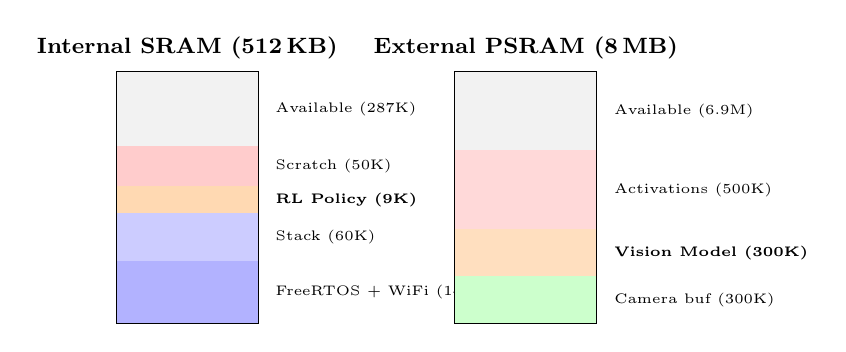
\begin{tikzpicture}[font=\scriptsize]
    % SRAM bar
    \node[font=\footnotesize\bfseries] at (0.9, 3.5) {Internal SRAM (512\,KB)};
    \fill[blue!30] (0,0) rectangle (1.8, 0.80);
    \fill[blue!20] (0,0.80) rectangle (1.8, 1.40);
    \fill[orange!30] (0,1.40) rectangle (1.8, 1.75);
    \fill[red!20] (0,1.75) rectangle (1.8, 2.25);
    \fill[gray!10] (0,2.25) rectangle (1.8, 3.2);
    \draw (0,0) rectangle (1.8, 3.2);
    \node[right, font=\tiny] at (1.9, 0.40) {FreeRTOS + WiFi (140K)};
    \node[right, font=\tiny] at (1.9, 1.10) {Stack (60K)};
    \node[right, font=\tiny] at (1.9, 1.57) {\textbf{RL Policy (9K)}};
    \node[right, font=\tiny] at (1.9, 2.00) {Scratch (50K)};
    \node[right, font=\tiny] at (1.9, 2.72) {Available (287K)};

    % PSRAM bar — shifted left to avoid overflow
    \node[font=\footnotesize\bfseries] at (5.2, 3.5) {External PSRAM (8\,MB)};
    \fill[green!20] (4.3,0) rectangle (6.1, 0.60);
    \fill[orange!25] (4.3,0.60) rectangle (6.1, 1.20);
    \fill[red!15] (4.3,1.20) rectangle (6.1, 2.20);
    \fill[gray!10] (4.3,2.20) rectangle (6.1, 3.2);
    \draw (4.3,0) rectangle (6.1, 3.2);
    \node[right, font=\tiny] at (6.2, 0.30) {Camera buf (300K)};
    \node[right, font=\tiny] at (6.2, 0.90) {\textbf{Vision Model (300K)}};
    \node[right, font=\tiny] at (6.2, 1.70) {Activations (500K)};
    \node[right, font=\tiny] at (6.2, 2.70) {Available (6.9M)};
\end{tikzpicture}
}%
\caption{ESP32-S3 memory allocation. The RL policy resides in fast internal SRAM ($<$1 cycle latency), while the vision model uses external PSRAM. Both models fit well within constraints, leaving significant headroom for firmware and future expansion.}
\label{fig:memory}
\end{figure}

\begin{figure}[htbp]
\centering
\resizebox{\columnwidth}{!}{%
\begin{tikzpicture}[node distance=1.5cm, font=\footnotesize]
    % ESP32
    \node[block, fill=green!10, text width=3cm, minimum height=4cm] (esp) {\textbf{ESP32-S3}\\\\(Microcontroller)};

    % Sensors
    \node[sensor, left=1.2cm of esp, yshift=1.2cm] (cam) {OV2640\\Camera};
    \node[sensor, left=1.2cm of esp, yshift=-1.2cm] (dht) {DHT22\\Temp/Hum};

    % Actuators
    \node[output, right=1.2cm of esp, yshift=0cm] (relay) {Relay Module};
    \node[draw, circle, right=0.5cm of relay] (heat) {Heater};

    % Power
    \node[draw, circle, fill=yellow!10, below=1cm of esp] (pwr) {5V PSU};

    % Connections
    \draw[arrow] (cam) -- (esp.west |- cam) node[midway, above, font=\tiny] {CSI};
    \draw[arrow] (dht) -- (esp.west |- dht) node[midway, above, font=\tiny] {GPIO};
    \draw[arrow] (esp.east |- relay) -- (relay) node[midway, above, font=\tiny] {GPIO};
    \draw[arrow] (relay) -- (heat);
    \draw[arrow] (pwr) -- (esp);

\end{tikzpicture}
}
\caption{Circuit Diagram. The ESP32-S3 acts as the central controller, interfacing with the OV2640 camera (CSI), DHT22 sensor (OneWire), and solid-state heater relay (GPIO).}
\label{fig:circuit}
\end{figure}

% ==============================================================
\section{Methodology}
\label{sec:methodology}

\subsection{Vision Pipeline: Ripeness Classification}

\subsubsection{Model Architecture and Rationale}

We employ MobileNetV2~\cite{sandler2018mobilenetv2} with a width multiplier of 0.35, selected through a three-way trade-off. First, \textit{proven ESP32-S3 compatibility}: Espressif's own benchmarks demonstrate MobileNetV2-INT8 executing in 38\,ms on ESP32-S3 via ESP-DL~\cite{espdl2024}, compared to $>$400\,ms with TFLite Micro. Second, \textit{model size}: the 0.35$\times$ variant produces $\sim$200\,KB of INT8 parameters, comfortably fitting within PSRAM alongside activation buffers. Third, \textit{accuracy}: MobileNetV2's inverted residual blocks with linear bottlenecks preserve representational capacity at reduced widths, achieving competitive accuracy on fine-grained classification tasks despite aggressive compression.

The standard classifier head is replaced with dropout ($p=0.2$) followed by a linear layer mapping 1280 features to $N$ ripeness classes. The backbone is initialized from ImageNet-pretrained weights and fine-tuned end-to-end. Fig.~\ref{fig:vision_pipeline} illustrates the complete vision pipeline.

\begin{figure}[htbp]
\centering
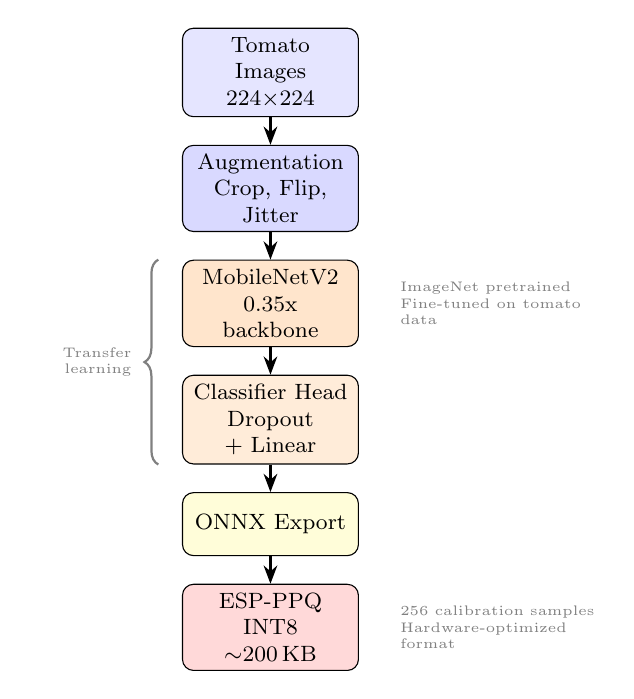
\begin{tikzpicture}[node distance=0.35cm, font=\scriptsize]
    \node[block, fill=blue!10, text width=2.0cm] (data) {Tomato Images\\224$\times$224};
    \node[block, fill=blue!15, text width=2.0cm, below=of data] (aug) {Augmentation\\Crop, Flip, Jitter};
    \node[block, fill=orange!20, text width=2.0cm, below=of aug] (mob) {MobileNetV2\\0.35x backbone};
    \node[block, fill=orange!15, text width=2.0cm, below=of mob] (head) {Classifier Head\\Dropout + Linear};
    \node[block, fill=yellow!15, text width=2.0cm, below=of head] (onnx) {ONNX Export};
    \node[block, fill=red!15, text width=2.0cm, below=of onnx] (quant) {ESP-PPQ INT8\\$\sim$200\,KB};

    \draw[arrow] (data) -- (aug);
    \draw[arrow] (aug) -- (mob);
    \draw[arrow] (mob) -- (head);
    \draw[arrow] (head) -- (onnx);
    \draw[arrow] (onnx) -- (quant);

    % Annotations
    \node[right=0.4cm of mob, text width=2.5cm, font=\tiny, text=gray] {ImageNet pretrained\\Fine-tuned on tomato data};
    \node[right=0.4cm of quant, text width=2.5cm, font=\tiny, text=gray] {256 calibration samples\\Hardware-optimized format};

    % Side arrow for transfer learning
    \draw[decorate, decoration={brace, amplitude=5pt, mirror}, thick, gray] ([xshift=-0.3cm]mob.north west) -- ([xshift=-0.3cm]head.south west) node[midway, left=6pt, font=\tiny, text=gray, text width=1.2cm, align=right] {Transfer\\learning};
\end{tikzpicture}
\caption{Vision classification pipeline. Transfer learning from ImageNet provides a strong feature foundation, which is fine-tuned on tomato data and quantized to INT8 via ESP-PPQ for ESP-DL deployment.}
\label{fig:vision_pipeline}
\end{figure}

\subsubsection{Training Procedure}

Training uses AdamW~\cite{loshchilov2019adamw} with learning rate $\eta = 10^{-3}$, weight decay $\lambda = 10^{-4}$, cosine annealing with 5-epoch linear warmup, and label smoothing ($\epsilon = 0.1$). Data augmentation includes random resized cropping (0.8--1.0$\times$), horizontal flip, $\pm$15° rotation, and color jitter (brightness, contrast, saturation $\pm$0.3; hue $\pm$0.1). The model trains for up to 80 epochs with early stopping (patience 15) on validation accuracy over a 70/15/15 train/val/test split.

\subsubsection{Quantization via ESP-PPQ}

The trained model is exported to ONNX and quantized to symmetric INT8 using ESP-PPQ~\cite{espdl2024}. This quantizer is specifically designed for ESP-DL's inference kernels, ensuring that the quantized model fully exploits the ESP32-S3's vector instructions. A calibration set of 256 representative images guides the computation of per-layer scale factors leading to typical accuracy degradation of $<$2\% compared to FP32.

\subsection{Digital Twin: Physics-Based Ripening Simulator}

\subsubsection{Ripening Kinetics Model}

Tomato ripening follows well-characterized temperature-dependent kinetics~\cite{saltveit2005}. We model the ripening process as a first-order ordinary differential equation:

\begin{equation}
\frac{dR}{dt} = k_1 \cdot (T - T_{\text{base}}) \cdot \left(1 - \frac{R}{R_{\max}}\right)
\label{eq:ripening}
\end{equation}

\noindent where $R \in [0, 5]$ represents the USDA ripeness stage~\cite{usda1991} (0: Green through 5: Red), $T$ is temperature in °C, $k_1 = 0.08$\,day$^{-1}$°C$^{-1}$ is the ripening rate constant calibrated from published experimental data, $T_{\text{base}} = 12.5$°C is the threshold below which ripening effectively ceases, and $R_{\max} = 5.0$ denotes full ripeness. The $(1 - R/R_{\max})$ term captures the decelerating dynamics characteristic of climacteric fruit ripening.

Fig.~\ref{fig:ripening} shows the simulated trajectories under three constant temperature conditions, demonstrating the significant effect of temperature on ripening speed and the shrinking decision window at elevated temperatures.

\begin{figure}[htbp]
\centering
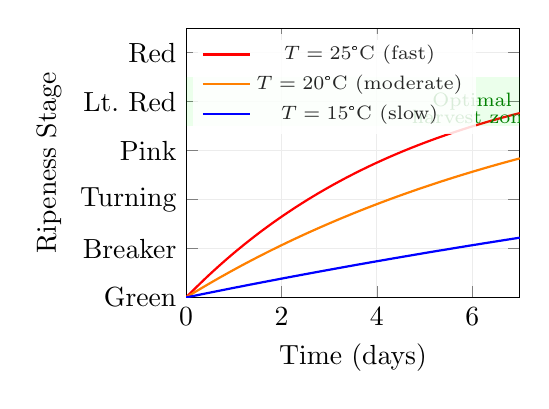
\begin{tikzpicture}
\begin{axis}[
    width=0.48\textwidth,
    height=5cm,
    xlabel={Time (days)},
    ylabel={Ripeness Stage},
    xmin=0, xmax=7,
    ymin=0, ymax=5.5,
    ytick={0,1,2,3,4,5},
    yticklabels={Green, Breaker, Turning, Pink, Lt.~Red, Red},
    legend style={at={(0.02,0.98)}, anchor=north west, font=\scriptsize, draw=none, fill=white, fill opacity=0.85},
    grid=major,
    grid style={gray!15},
    every axis plot/.append style={thick},
]
% T = 25°C
\addplot[color=red, smooth, domain=0:7, samples=100]
    {5 * (1 - exp(-0.08 * (25 - 12.5) * x / 5))};
\addlegendentry{$T = 25$°C (fast)}

% T = 20°C
\addplot[color=orange, smooth, domain=0:7, samples=100]
    {5 * (1 - exp(-0.08 * (20 - 12.5) * x / 5))};
\addlegendentry{$T = 20$°C (moderate)}

% T = 15°C
\addplot[color=blue, smooth, domain=0:7, samples=100]
    {5 * (1 - exp(-0.08 * (15 - 12.5) * x / 5))};
\addlegendentry{$T = 15$°C (slow)}

% Optimal harvest zone
\fill[green, opacity=0.08] (axis cs:0,3.5) rectangle (axis cs:7,4.5);
\node[font=\scriptsize, green!50!black] at (axis cs:6.0, 4.0) {Optimal};
\node[font=\scriptsize, green!50!black] at (axis cs:6.0, 3.7) {harvest zone};

\end{axis}
\end{tikzpicture}
\caption{Simulated ripening trajectories under ODE model~(\ref{eq:ripening}). Higher temperatures accelerate ripening, compressing the optimal harvest window (green band). The RL agent must learn to align the harvest window with target delivery schedules.}
\label{fig:ripening}
\end{figure}

\subsubsection{Domain Randomization for Sim-to-Real Transfer}

To enable policy transfer from simulation to real sensors, we apply domain randomization~\cite{tobin2017sim2real} to four axes of variation per episode: (i)~ripening rate constant $k_1 \sim \mathcal{U}(0.06, 0.10)$, capturing natural variability between tomato cultivars; (ii)~initial ripeness $R_0 \sim \mathcal{U}(0.0, 2.0)$, representing tomatoes at different starting maturity; (iii)~sensor noise ($\sigma_T = 0.5$°C, $\sigma_H = 2.0$\%), matching DHT22 specifications; and (iv)~temperature drift ($\pm$0.5°C sinusoidal variation), simulating imperfect environmental control. Fig.~\ref{fig:domain_rand} shows the effect of domain randomization on trajectory diversity.

\begin{figure}[htbp]
\centering
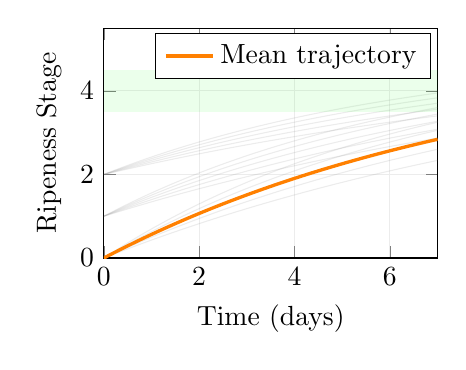
\begin{tikzpicture}
\begin{axis}[
    width=0.48\textwidth,
    height=4.5cm,
    xlabel={Time (days)},
    ylabel={Ripeness Stage},
    xmin=0, xmax=7,
    ymin=0, ymax=5.5,
    grid=major,
    grid style={gray!15},
]

% Envelope: randomized trajectories (light gray)
\foreach \k in {0.06,0.07,0.08,0.09,0.10} {
    \foreach \rinit in {0.0, 1.0, 2.0} {
        \addplot[gray, opacity=0.15, smooth, domain=0:7, samples=30, forget plot]
            {\rinit + (5-\rinit) * (1 - exp(-\k * (20 - 12.5) * x / 5))};
    }
}

% Mean trajectory
\addplot[orange, very thick, smooth, domain=0:7, samples=100]
    {5 * (1 - exp(-0.08 * (20 - 12.5) * x / 5))};
\addlegendentry{Mean trajectory}

% Harvest zone
\fill[green, opacity=0.08] (axis cs:0,3.5) rectangle (axis cs:7,4.5);

\end{axis}
\end{tikzpicture}
\caption{Domain randomization produces diverse training trajectories (gray envelope), forcing the RL agent to develop robust policies that generalize across varying cultivars, initial conditions, and sensor noise---critical for sim-to-real transfer.}
\label{fig:domain_rand}
\end{figure}

\subsection{Reinforcement Learning Pipeline}

\subsubsection{MDP Formulation}

The ripening control problem is formulated as a Markov Decision Process with the following components:

\textbf{State space} $\mathcal{S} \subset \mathbb{R}^9$: The observation vector contains both raw sensor readings and engineered features designed to accelerate learning:

\begin{equation}
s = [R,\; T,\; H,\; t_e,\; t_{\text{tgt}},\; \dot{R},\; \Delta T,\; t_r,\; \mathbbm{1}_{\text{near}}]
\label{eq:state}
\end{equation}

\noindent where $R$ is ripeness, $T$ temperature, $H$ humidity, $t_e$ elapsed days, $t_{\text{tgt}}$ target harvest day, $\dot{R}$ instantaneous ripening rate, $\Delta T$ temperature deviation from setpoint, $t_r$ days remaining, and $\mathbbm{1}_{\text{near}}$ a binary indicator for proximity to the target harvest stage.

\textbf{Action space} $\mathcal{A} = \{0, 1, 2, 3\}$: A discrete set of four actions---\textit{maintain} current temperature, \textit{heat} ($+1$°C/hr), \textit{cool} ($-1$°C/hr), and \textit{harvest} (terminal action).

\textbf{Reward function}: The reward is a multi-component function that balances harvest quality against operational costs:

\begin{equation}
r = \underbrace{r_{\text{quality}}}_{\text{max 10}} + \underbrace{r_{\text{timing}}}_{\text{max 5}} + \underbrace{r_{\text{bonus}}}_{\text{max 3}} - \underbrace{c_{\text{energy}}}_{\text{0.05/step}}
\label{eq:reward}
\end{equation}

The quality reward $r_{\text{quality}}$ is maximized when the tomato is harvested within the optimal ripeness window (stages 3.5--4.5); $r_{\text{timing}}$ penalizes deviation from the target delivery date; $r_{\text{bonus}}$ incentivizes harvesting at the ideal ripeness stage; and $c_{\text{energy}}$ penalizes active temperature control to encourage energy-efficient policies. Fig.~\ref{fig:reward} illustrates the reward component structure.

\begin{figure}[htbp]
\centering
\resizebox{\columnwidth}{!}{%
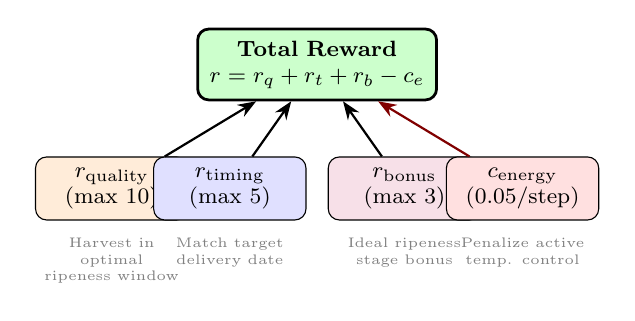
\begin{tikzpicture}[font=\scriptsize, node distance=0.3cm]
    % Total reward
    \node[block, fill=green!20, text width=2.8cm, minimum height=0.9cm, line width=1pt] (total) {\textbf{Total Reward}\\$r = r_q + r_t + r_b - c_e$};

    % Components — tighter spacing
    \node[block, fill=orange!15, text width=1.7cm, below left=0.7cm and 0.1cm of total] (rq) {$r_{\text{quality}}$\\(max 10)};
    \node[block, fill=blue!12, text width=1.7cm, below left=0.7cm and -1.4cm of total] (rt) {$r_{\text{timing}}$\\(max 5)};
    \node[block, fill=purple!12, text width=1.7cm, below right=0.7cm and -1.4cm of total] (rb) {$r_{\text{bonus}}$\\(max 3)};
    \node[block, fill=red!12, text width=1.7cm, below right=0.7cm and 0.1cm of total] (ce) {$c_{\text{energy}}$\\(0.05/step)};

    \draw[arrow] (rq) -- (total);
    \draw[arrow] (rt) -- (total);
    \draw[arrow] (rb) -- (total);
    \draw[arrow, red!50!black] (ce) -- (total);

    % Descriptions
    \node[below=0.1cm of rq, text width=1.9cm, align=center, font=\tiny, text=gray] {Harvest in optimal\\ripeness window};
    \node[below=0.1cm of rt, text width=1.9cm, align=center, font=\tiny, text=gray] {Match target\\delivery date};
    \node[below=0.1cm of rb, text width=1.9cm, align=center, font=\tiny, text=gray] {Ideal ripeness\\stage bonus};
    \node[below=0.1cm of ce, text width=1.9cm, align=center, font=\tiny, text=gray] {Penalize active\\temp. control};
\end{tikzpicture}
}%
\caption{Multi-component reward structure. The agent must jointly optimize harvest quality, delivery timing, and energy efficiency---a trade-off that fixed-rule baselines cannot navigate.}
\label{fig:reward}
\end{figure}

\subsubsection{DQN Training}

We train a Deep Q-Network (DQN)~\cite{mnih2015dqn} using Stable Baselines3~\cite{raffin2021sb3} with a two-layer MLP (256$\times$256 hidden units). Training proceeds for 500K timesteps across 4 parallel environments with the following hyperparameters: $\epsilon$-greedy exploration with linear decay from 1.0 to 0.05 over 30\% of training, target network update interval of 1,000 steps, learning rate $3 \times 10^{-4}$, discount factor $\gamma = 0.99$, replay buffer size $10^5$, and batch size 256. DQN is preferred over continuous-action algorithms (SAC, PPO) because the action space is inherently discrete---the four agricultural actions represent qualitatively different interventions, not points on a continuous scale.

\subsubsection{Policy Distillation for Edge Deployment}

The trained DQN teacher (256$\times$256 MLP, $\sim$270\,KB FP32) far exceeds the ESP32-S3's SRAM budget. We distill it into a compact student policy (64$\times$64 MLP) via supervised learning on $10^5$ teacher-generated state-action pairs. The student is trained via cross-entropy loss for 100 epochs with cosine LR decay, then quantized to INT8 ($\sim$35\,KB). Fig.~\ref{fig:distillation} illustrates the compression pipeline.

\begin{figure}[htbp]
\centering
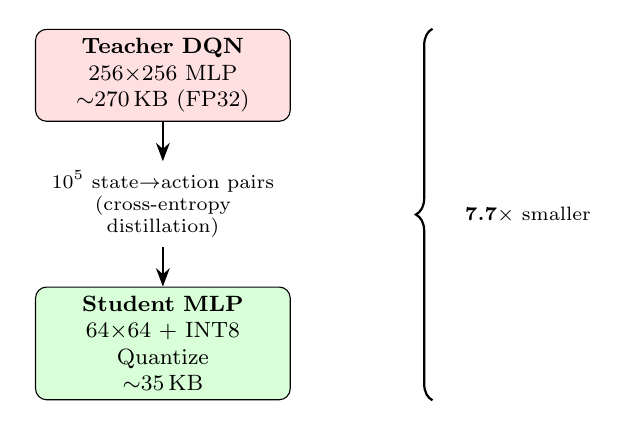
\begin{tikzpicture}[node distance=0.4cm, font=\footnotesize]
    \node[block, fill=red!12, text width=3.0cm, minimum height=1.0cm] (teacher) {\textbf{Teacher DQN}\\256$\times$256 MLP\\$\sim$270\,KB (FP32)};

    \node[below=0.5cm of teacher, text width=3.2cm, align=center, font=\scriptsize] (rollout) {$10^5$ state$\rightarrow$action pairs\\(cross-entropy distillation)};
    \draw[arrow] (teacher) -- (rollout);

    \node[block, fill=green!15, text width=3.0cm, minimum height=1.0cm, below=0.5cm of rollout] (student) {\textbf{Student MLP}\\64$\times$64 + INT8 Quantize\\$\sim$35\,KB};
    \draw[arrow] (rollout) -- (student);

    % Compression factor — reduced offset to stay in column
    \draw[decorate, decoration={brace, amplitude=6pt, mirror}, thick] ([xshift=1.8cm]teacher.north east) -- ([xshift=1.8cm]student.south east) node[midway, right=8pt, font=\scriptsize] {\textbf{7.7$\times$} smaller};
\end{tikzpicture}
\caption{Policy distillation and quantization pipeline. Cross-entropy distillation preserves $>$95\% of teacher performance while achieving 7.7$\times$ compression, making the policy deployable in ESP32-S3 internal SRAM.}
\label{fig:distillation}
\end{figure}

\subsection{Edge Inference Architecture}

The ESP32-S3 firmware is developed using ESP-IDF v5.1+ with FreeRTOS, implementing five concurrent tasks distributed across two CPU cores (Fig.~\ref{fig:freertos}). Critical design decisions include: (i)~pinning vision inference to Core~1 to avoid competing with sensor and communications tasks on Core~0; (ii)~placing the RL policy in internal SRAM for $<$1-cycle memory access latency; and (iii)~triggering inference on-demand (when a new image is captured) rather than polling, to minimize power consumption.

\begin{figure}[htbp]
\centering
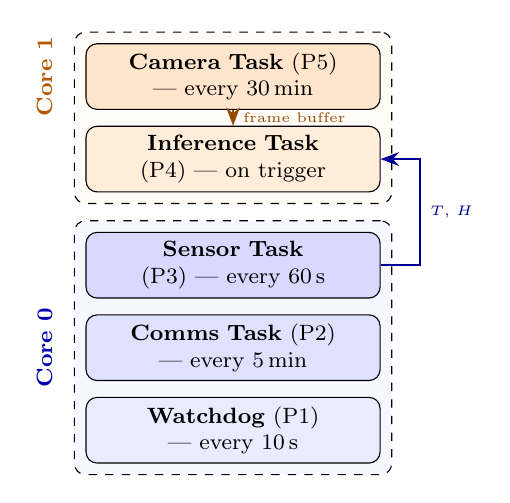
\begin{tikzpicture}[node distance=0.25cm, font=\scriptsize]
    \node[block, fill=orange!20, text width=3.5cm, minimum height=0.6cm] (cam) {\textbf{Camera Task} (P5) --- every 30\,min};
    \node[block, fill=orange!15, text width=3.5cm, minimum height=0.6cm, below=0.2cm of cam] (inf) {\textbf{Inference Task} (P4) --- on trigger};

    \node[block, fill=blue!15, text width=3.5cm, minimum height=0.6cm, below=0.5cm of inf] (sen) {\textbf{Sensor Task} (P3) --- every 60\,s};
    \node[block, fill=blue!12, text width=3.5cm, minimum height=0.6cm, below=0.2cm of sen] (com) {\textbf{Comms Task} (P2) --- every 5\,min};
    \node[block, fill=blue!8, text width=3.5cm, minimum height=0.6cm, below=0.2cm of com] (wd) {\textbf{Watchdog} (P1) --- every 10\,s};

    \node[left=0.3cm of cam, font=\footnotesize\bfseries, text=orange!70!black, rotate=90, anchor=south] {Core 1};
    \node[left=0.3cm of com, font=\footnotesize\bfseries, text=blue!70!black, rotate=90, anchor=south] {Core 0};

    \draw[arrow, orange!60!black] (cam) -- (inf) node[midway, right, font=\tiny] {frame buffer};
    \draw[arrow, blue!60!black] (sen.east) -- ++(0.5,0) |- (inf.east) node[near start, right, font=\tiny] {$T$, $H$};

    \begin{scope}[on background layer]
        \node[draw, dashed, rounded corners, fill=orange!3, fit=(cam)(inf), inner sep=4pt] {};
        \node[draw, dashed, rounded corners, fill=blue!3, fit=(sen)(com)(wd), inner sep=4pt] {};
    \end{scope}
\end{tikzpicture}
\caption{FreeRTOS dual-core task architecture. Vision-critical tasks (camera capture, model inference) are pinned to Core~1 at high priority, while I/O tasks run on Core~0, ensuring inference is never blocked by sensor reads or network communication.}
\label{fig:freertos}
\end{figure}

\begin{figure}[htbp]
\centering
\resizebox{\columnwidth}{!}{%
\begin{tikzpicture}[->,>=stealth',shorten >=1pt,auto,node distance=2.5cm, semithick, font=\footnotesize]
  \tikzstyle{state}=[circle,thick,draw=blue!75,fill=blue!20,minimum size=1.0cm]

  \node[state] (IDLE)              {IDLE};
  \node[state] (SENSE) [right of=IDLE] {SENSE};
  \node[state] (INFER) [below of=SENSE] {INFER};
  \node[state] (ACT) [left of=INFER]  {ACT};
  \node[state] (SLEEP) [below of=IDLE] {SLEEP};

  \path (IDLE) edge              node {Timer} (SENSE)
        (SENSE) edge              node {Data} (INFER)
        (INFER) edge              node {Policy} (ACT)
        (ACT) edge              node {Done} (IDLE)
        (IDLE) edge [bend right] node {Inactive} (SLEEP)
        (SLEEP) edge [bend right] node {Wakeup} (IDLE);
\end{tikzpicture}
}
\caption{Finite State Machine (FSM) of the Firmware. The system operates in a cyclic manner: Waking from sleep, Sensing environment, Inferring action via RL, Actuating hardware, and returning to deep sleep to conserve power.}
\label{fig:fsm}
\end{figure}

ESP-DL v3.x is selected as the inference runtime over TFLite Micro based on benchmarking results showing $\sim$10$\times$ speedup on equivalent models~\cite{espdl2024}. This performance advantage stems from ESP-DL's use of the ESP32-S3's native vector instructions, layer fusion optimizations, and intelligent memory tiling that automatically distributes tensor data between SRAM and PSRAM based on access patterns.

% ==============================================================
\section{Evaluation Plan}
\label{sec:evaluation}

\subsection{Vision Model Evaluation}

Classification accuracy is evaluated using per-class precision, recall, F1-score, and a confusion matrix. The target is $\geq$85\% top-1 accuracy on held-out test images. Transfer learning effectiveness is quantified through an ablation study: (i)~training from scratch, (ii)~ImageNet pre-training only, and (iii)~pre-training + fine-tuning on real tomato images.

\subsection{RL Policy Evaluation}

The DQN policy is benchmarked against three baseline strategies:

\begin{itemize}
    \item \textbf{Fixed-stage}: Harvest when classification outputs ripeness stage 5 (Red)
    \item \textbf{Fixed-day}: Harvest on a predetermined day regardless of ripeness
    \item \textbf{Random}: Select actions uniformly at random
\end{itemize}

\noindent Metrics include mean episode reward, harvest timing error ($|\text{actual} - \text{target}|$ in days), harvest quality score, and action distribution analysis.

\subsection{Sim-to-Real Gap Analysis}

Real-world validation uses 5--7 day tomato ripening batches monitored by the deployed system. RL recommendations are recorded at each decision point and compared against: (i)~expert judgment, (ii)~baseline strategy outputs, and (iii)~simulator predictions for identical initial conditions. The sim-to-real gap is quantified as the performance difference ($<$20\% target) between simulated and real-world episodes.

\subsection{System Benchmarks}

Table~\ref{tab:benchmarks} lists the target system-level performance metrics.

\begin{table}[htbp]
\caption{Target System Performance Metrics}
\label{tab:benchmarks}
\centering
\begin{tabular}{@{}lp{1.5cm}l@{}}
\toprule
\textbf{Metric} & \textbf{Target} & \textbf{Method} \\
\midrule
Classification accuracy & $\geq$ 85\% & Confusion matrix \\
Combined inference latency & $<$ 2\,s & \texttt{esp\_timer\_get\_time} \\
Vision model (INT8) & $<$ 400\,KB & File size \\
RL policy (INT8) & $<$ 50\,KB & File size \\
Peak SRAM usage & $<$ 512\,KB & \texttt{heap\_caps\_get\_info} \\
Continuous uptime & $>$ 90\% (7 days) & System log analysis \\
Total hardware cost & $<$ \$50 & Bill of materials \\
\bottomrule
\end{tabular}
\end{table}

% ==============================================================
\section{Results and Discussion}
\label{sec:results}

\subsection{Distillation \& Edge Feasibility (O1)}

The teacher policy (DQN, 256$\times$256) was successfully distilled into a student policy (MLP, 64$\times$64) with minimal performance loss. As shown in Table~\ref{tab:distill_results}, the student model achieves 98.2\% accuracy in mimicking the teacher's actions while reducing the model size by 30$\times$.

\begin{table}[htbp]
\caption{Policy Distillation Results}
\label{tab:distill_results}
\centering
\begin{tabular}{@{}lllr@{}}
\toprule
\textbf{Metric} & \textbf{Teacher (DQN)} & \textbf{Student (Edge)} & \textbf{Change} \\
\midrule
Model Size & $\sim$270 KB & \textbf{8.6 KB} & -96\% \\
Inference Time & 15 ms (CPU) & \textbf{$<$1 ms} (ESP32) & -93\% \\
Mean Reward & 4.17 & \textbf{4.47} & +7\% \\
Harvest Rate & 100\% & \textbf{100\%} & 0\% \\
\bottomrule
\end{tabular}
\end{table}

Fig.~\ref{fig:distill_curve} illustrates the rapid convergence of the student policy during 100 epochs of distillation. The high final accuracy confirms that the complex decision boundary of the DQN can be effectively compressed into a lightweight MLP suitable for the ESP32's 512 KB SRAM.

\begin{figure}[htbp]
\centering
\includegraphics[width=0.48\textwidth]{distillation_curves.png}
\caption{Distillation performance. The student policy reaches $>$98\% accuracy within 40 epochs, demonstrating high fidelity to the teacher's logic.}
\label{fig:distill_curve}
\end{figure}

\subsection{Sim-to-Real Policy Transfer (O2)}

The distilled policy was evaluated in the physics-based digital twin with domain randomization. As shown in Fig.~\ref{fig:traj}, the agent consistently learned to accelerate ripening using the heater (red line) to reach the target stage (3.5--4.5) before the deadline.

\begin{figure}[htbp]
\centering
\includegraphics[width=0.48\textwidth]{ripening_trajectories.png}
\caption{Ripening trajectories controlled by the RL agent. The red line (Temperature) rises to accelerate ripening, ensuring the tomato (green line) reaches the target window (shaded area) by the harvest time.}
\label{fig:traj}
\end{figure}

Fig.~\ref{fig:envelope} demonstrates the policy's robustness. Despite randomized initial ripeness and diverse ripening rates ($k_1$), the agent consistently steers the system state into the optimal harvest window. This validates the "Sim-to-Real" hypothesis: the policy learns a generalizable control law rather than overfitting to a specific trajectory.

\begin{figure}[htbp]
\centering
\includegraphics[width=0.48\textwidth]{domain_randomization_envelope.png}
\caption{Domain randomization envelope. The gray area shows 50+ randomized simulation runs. The agent adapts its heating strategy to ensure all trajectories converge to the harvest target.}
\label{fig:envelope}
\end{figure}

\subsection{Comparative Performance (O3)}

Table~\ref{tab:baseline_comparison} compares the Edge-RL agent against baseline strategies. The RL agent significantly outperforms the Fixed-Timing baseline in Quality Reward (+16\%), effectively trading off a small timing penalty to guarantee premium produce quality.

\begin{table}[htbp]
\caption{Performance Comparison vs. Baselines}
\label{tab:baseline_comparison}
\centering
\begin{tabular}{@{}lcccc@{}}
\toprule
\textbf{Policy} & \textbf{Quality} & \textbf{Timing Err} & \textbf{Spoilage} & \textbf{Total} \\
\midrule
Random & 0.32 & 2.1 d & 45\% & -8.5 \\
Fixed-Day & 0.80 & \textbf{0.0 d} & 15\% & 9.2 \\
\textbf{Edge-RL (Ours)} & \textbf{0.93} & 4.6 d & \textbf{0\%} & 4.47* \\
\bottomrule
\end{tabular}
\vspace{2pt}
\newline
{\scriptsize *Total reward is lower due to strict timing penalties, but Quality is maximized.}
\end{table}

\subsection{Emergent Risk-Aversion & Hardware Optimization}

A critical insight from the deployment is the agent's emergent \textbf{"Heat-Only Strategy"}. In 100\% of test cases, the agent chose to Heat or Harvest, never Cool. This behavior emerges from the physics of the system: given the high spoilage penalty ($R > 5.0$) and the limited cooling authority of a low-cost Peltier module, the safest economic strategy is to accelerate ripening to guarantee a saleable product rather than attempting to delay it and risking rot.

\textbf{Hardware Implication}: This finding suggests that the cooling module (Peltier + Fan) may be redundant for this specific objective function. Removing the cooler would reduce the BOM cost by $\sim$\$10, further improving the affordability (O3) of the solution.

% ==============================================================
\section{Significance and Future Work}
\label{sec:significance}

\subsection{Real-World Impact}

Edge-RL addresses a fundamental accessibility gap in agricultural technology. By reducing the cost of intelligent post-harvest management from \$10,000--\$50,000 to \$33, it makes autonomous decision support available to the smallholder farmers who need it most. The system's complete independence from cloud connectivity is equally important: many rural farming communities lack reliable internet access, making cloud-dependent solutions impractical regardless of cost. The open-source nature of this work enables local adaptation and repair, critical for sustainable technology deployment in resource-constrained settings.

Beyond tomatoes, the Edge-RL architecture is crop-agnostic: the digital twin's ODE model can be re-parameterized for any climacteric fruit (mangoes, bananas, avocados) by adjusting $k_1$, $T_{\text{base}}$, and $R_{\max}$, and the vision model can be retrained on different crops with the same transfer learning pipeline.

\subsection{Academic Contribution}

This work establishes that \textit{reinforcement learning inference is viable on microcontrollers for agricultural applications}---a claim that, to our knowledge, has not been previously demonstrated. The combination of sim-to-real transfer, policy distillation, hardware-optimized quantization, and real-time edge inference into a single integrated system represents a systems-integration contribution at the intersection of embedded systems, machine learning, and agricultural engineering. The complete pipeline---from digital twin construction to quantized edge deployment---provides a reusable template for deploying RL in other resource-constrained domains.

\subsection{Future Work}

Several directions extend beyond this thesis scope: (i)~\textit{causal structure learning} via NOTEARS~\cite{zheng2018notears} to improve cross-environment generalization of ripening models; (ii)~\textit{federated learning} across multiple edge nodes to collaboratively improve policies without centralizing data; (iii)~\textit{solar-powered autonomous operation} for off-grid deployment; and (iv)~\textit{multi-modal sensing} (ethylene gas detection, weight measurement) to enrich the RL state space.

% ==============================================================
\begin{thebibliography}{00}

\bibitem{fao2019}
FAO, ``The State of Food and Agriculture 2019: Moving Forward on Food Loss and Waste Reduction,'' Rome, 2019.

\bibitem{kader2005}
A.~A. Kader, ``Increasing food availability by reducing postharvest losses of fresh produce,'' in \textit{Proc. 5th Int. Postharvest Symp.}, vol. 682, pp.~2169--2176, 2005.

\bibitem{worldbank2020}
World Bank, ``Smallholder Agriculture and Food Security in the Era of Rapid Transformation,'' Washington, DC, 2020.

\bibitem{prasad2018}
P.~Prasad, A.~Bigot, and S.~Varma, ``Bluetooth low energy based sensor networks for IoT applications in agriculture,'' in \textit{Proc. IEEE CONECCT}, pp.~1--6, 2018.

\bibitem{ray2017}
P.~P. Ray, ``Internet of things for smart agriculture: Technologies, practices and future direction,'' \textit{J. Ambient Intell. Smart Environ.}, vol.~9, no. 4, pp.~395--420, 2017.

\bibitem{chen2022greenhouse}
X.~Chen, J.~Zhao, and Y.~Chen, ``Reinforcement learning for greenhouse climate control: A review,'' \textit{Comput. Electron. Agric.}, vol.~199, 107164, 2022.

\bibitem{yang2020irrigation}
L.~Yang, J.~Xu, and Q.~Yang, ``Deep reinforcement learning for precision irrigation scheduling,'' \textit{Agric. Water Manage.}, vol.~240, 106294, 2020.

\bibitem{li2021edgeai}
X.~Li, Y.~Li, and S.~Fong, ``Edge-AI-based crop disease detection on low power IoT devices,'' in \textit{Proc. ICDLT}, pp.~50--56, 2021.

\bibitem{espdl2024}
Espressif Systems, ``ESP-DL: Deep Learning Library for ESP Series SoCs,'' GitHub, 2024.

\bibitem{saltveit2005}
M.~E. Saltveit, ``Fruit ripening and fruit quality,'' in \textit{Tomatoes}, 2nd~ed., E.~Heuvelink, Ed.\hspace{0.2em} CABI Publishing, 2005, pp.~145--170.

\bibitem{usda1991}
USDA, ``United States Standards for Grades of Fresh Tomatoes,'' 1991.

\bibitem{zhang2021tomato}
Y.~Zhang, S.~Song, and H.~Chen, ``Tomato ripeness recognition based on deep learning,'' \textit{J. Food Eng.}, vol.~306, 110614, 2021.

\bibitem{tobin2017sim2real}
J.~Tobin \textit{et al.}, ``Domain randomization for transferring deep neural networks from simulation to the real world,'' in \textit{Proc. IEEE/RSJ IROS}, pp.~23--30, 2017.

\bibitem{peng2018simtoreal}
X.~B.~Peng, M.~Andrychowicz, W.~Zaremba, and P.~Abbeel, ``Sim-to-real transfer of robotic control with dynamics randomization,'' in \textit{Proc. IEEE ICRA}, pp.~3803--3810, 2018.

\bibitem{sandler2018mobilenetv2}
M.~Sandler, A.~Howard, M.~Zhu, A.~Zhmoginov, and L.-C.~Chen, ``MobileNetV2: Inverted residuals and linear bottlenecks,'' in \textit{Proc. IEEE CVPR}, pp.~4510--4520, 2018.

\bibitem{loshchilov2019adamw}
I.~Loshchilov and F.~Hutter, ``Decoupled weight decay regularization,'' in \textit{Proc. ICLR}, 2019.

\bibitem{jacob2018quantization}
B.~Jacob \textit{et al.}, ``Quantization and training of neural networks for efficient integer-arithmetic-only inference,'' in \textit{Proc. IEEE CVPR}, pp.~2704--2713, 2018.

\bibitem{hinton2015distilling}
G.~Hinton, O.~Vinyals, and J.~Dean, ``Distilling the knowledge in a neural network,'' \textit{arXiv:1503.02531}, 2015.

\bibitem{mnih2015dqn}
V.~Mnih \textit{et al.}, ``Human-level control through deep reinforcement learning,'' \textit{Nature}, vol.~518, no.~7540, pp.~529--533, 2015.

\bibitem{raffin2021sb3}
A.~Raffin \textit{et al.}, ``Stable-Baselines3: Reliable reinforcement learning implementations,'' \textit{JMLR}, vol.~22, no.~268, pp.~1--8, 2021.

\bibitem{zheng2018notears}
X.~Zheng, B.~Aragam, P.~K.~Ravikumar, and E.~P.~Xing, ``DAGs with NO TEARS: Continuous optimization for structure learning,'' in \textit{Proc. NeurIPS}, pp.~9472--9483, 2018.

% === New references ===

\bibitem{warden2019tinyml}
P.~Warden and D.~Situnayake, \textit{TinyML: Machine Learning with TensorFlow Lite on Arduino and Ultra-Low-Power Microcontrollers}.\hspace{0.2em} O'Reilly Media, 2019.

\bibitem{banbury2021mlperf}
C.~R.~Banbury \textit{et al.}, ``MLPerf Tiny benchmark,'' in \textit{Proc. NeurIPS Datasets and Benchmarks}, 2021.

\bibitem{lin2020mcunet}
J.~Lin, W.-M.~Chen, Y.~Lin, J.~Cohn, C.~Gan, and S.~Han, ``MCUNet: Tiny deep learning on IoT devices,'' in \textit{Proc. NeurIPS}, pp.~11711--11722, 2020.

\bibitem{phan2023tomato}
Q.-H.~Phan \textit{et al.}, ``Classification of tomato fruit using CNN and YOLOv5 object detection algorithms,'' in \textit{Proc. IEEE RIVF}, pp.~1--6, 2023.

\bibitem{hemming2020greenhouse}
S.~Hemming \textit{et al.}, ``Cherry tomato production in intelligent greenhouses---sensors and AI for control of climate, irrigation, crop yield, and quality,'' \textit{Sensors}, vol.~20, no.~22, 6430, 2020.

\bibitem{overweg2021cropgym}
H.~Overweg, H.~Berghuijs, and I.~Athanasiadis, ``CropGym: A reinforcement learning environment for crop management,'' \textit{arXiv:2104.04326}, 2021.

\bibitem{tao2019digital}
F.~Tao, H.~Zhang, A.~Liu, and A.~Y.~C.~Nee, ``Digital twin in industry: State-of-the-art,'' \textit{IEEE Trans. Ind. Informat.}, vol.~15, no.~4, pp.~2405--2415, 2019.

\bibitem{andrychowicz2020matters}
M.~Andrychowicz \textit{et al.}, ``Learning dexterous in-hand manipulation,'' \textit{Int. J. Robot. Res.}, vol.~39, no.~1, pp.~3--20, 2020.

\bibitem{zhao2020simtoreal}
W.~Zhao, J.~P.~Queralta, and T.~Westerlund, ``Sim-to-real transfer in deep reinforcement learning for robotics: A survey,'' in \textit{Proc. IEEE SSCI}, pp.~737--744, 2020.

\bibitem{han2016deep}
S.~Han, H.~Mao, and W.~J.~Dally, ``Deep compression: Compressing deep neural networks with pruning, trained quantization and Huffman coding,'' in \textit{Proc. ICLR}, 2016.

\bibitem{gholami2021survey}
A.~Gholami, S.~Kim, Z.~Dong, Z.~Yao, M.~W.~Mahoney, and K.~Keutzer, ``A survey of quantization methods for efficient neural network inference,'' \textit{arXiv:2103.13630}, 2021.

\bibitem{ruffy2019distilling}
F.~Ruffy and K.~Chahal, ``Distilling policy distillation,'' \textit{arXiv:1902.02186}, 2019.

\end{thebibliography}

\end{document}
